\documentclass[12pt,a4paper]{article}

% Paquetes
\usepackage[spanish]{babel}
\usepackage[utf8]{inputenc}
\usepackage[T1]{fontenc}
\usepackage{graphicx}
\usepackage{geometry}
\usepackage{fancyhdr}
\usepackage{hyperref}
\usepackage{xcolor}
\usepackage{tcolorbox}
\usepackage{enumitem}
\usepackage{booktabs}
\usepackage{float}
\usepackage{amssymb}

% Configuración de página
\geometry{
    left=2.5cm,
    right=2.5cm,
    top=3cm,
    bottom=3cm,
    headheight=14pt
}

% Colores personalizados
\definecolor{covidred}{RGB}{255,107,107}
\definecolor{normalgreen}{RGB}{81,207,102}
\definecolor{virusyellow}{RGB}{255,212,59}
\definecolor{primaryblue}{RGB}{41,128,185}

% Configuración de hipervínculos
\hypersetup{
    colorlinks=true,
    linkcolor=primaryblue,
    filecolor=primaryblue,
    urlcolor=primaryblue,
    citecolor=primaryblue
}

% Encabezado y pie de página
\pagestyle{fancy}
\fancyhf{}
\fancyhead[L]{\small Manual de Usuario - Sistema de Detección COVID-19}
\fancyhead[R]{\small Versión 15}
\fancyfoot[C]{\thepage}
\renewcommand{\headrulewidth}{0.4pt}
\renewcommand{\footrulewidth}{0.4pt}

% Comandos personalizados
\newcommand{\paso}[1]{\textbf{\textcolor{primaryblue}{#1}}}
\newcommand{\boton}[1]{\colorbox{gray!20}{\texttt{#1}}}
\newcommand{\nota}[1]{%
    \begin{tcolorbox}[colback=blue!5!white,colframe=primaryblue,title=Nota]
        #1
    \end{tcolorbox}
}
\newcommand{\advertencia}[1]{%
    \begin{tcolorbox}[colback=red!5!white,colframe=red,title=Importante]
        #1
    \end{tcolorbox}
}
\newcommand{\consejo}[1]{%
    \begin{tcolorbox}[colback=green!5!white,colframe=green!60!black,title=Consejo]
        #1
    \end{tcolorbox}
}

% Información del documento
\title{\Huge \textbf{Manual de Usuario} \\[0.5cm]
       \Large Sistema de Detección de COVID-19 \\
       mediante Análisis de Radiografías de Tórax \\[0.3cm]
       \large Versión 15}
\author{}
\date{Enero 2026}

\begin{document}

\maketitle
\thispagestyle{empty}

\vspace{2cm}

\begin{center}
\includegraphics[width=0.6\textwidth]{imagenes/portada_sistema.png}
\\[0.5cm]
\textit{Interfaz Web para Análisis Automático de Radiografías}
\end{center}

\newpage

\tableofcontents
\newpage

% ============================================================================
% CAPÍTULO 1: INTRODUCCIÓN
% ============================================================================
\section{Introducción}

\subsection{¿Qué es este sistema?}

Este manual le guiará en el uso del \textbf{Sistema de Detección de COVID-19}, una herramienta que analiza radiografías de tórax para identificar posibles casos de COVID-19, neumonía viral o pulmones normales.

El sistema utiliza tecnología de inteligencia artificial para:
\begin{itemize}[leftmargin=*]
    \item Detectar automáticamente puntos de referencia en los pulmones
    \item Normalizar la imagen para un análisis más preciso
    \item Clasificar la radiografía en una de tres categorías:
    \begin{itemize}
        \item \textcolor{covidred}{\textbf{COVID-19}}
        \item \textcolor{normalgreen}{\textbf{Normal}}
        \item \textcolor{virusyellow}{\textbf{Neumonía Viral}}
    \end{itemize}
    \item Mostrar resultados visuales fáciles de interpretar
\end{itemize}

\subsection{¿Para quién es este manual?}

Este manual está diseñado para usuarios \textbf{sin conocimientos técnicos previos}. No necesita saber de programación ni de computación avanzada para usar el sistema.

\subsection{¿Qué necesito para usar el sistema?}

\begin{itemize}[leftmargin=*]
    \item Una computadora con Windows
    \item Conexión a internet (solo para descargar el sistema)
    \item Radiografías de tórax en formato digital (PNG o JPG)
    \item Aproximadamente 10 minutos para la instalación inicial
\end{itemize}

\advertencia{
\textbf{Aviso importante:} Este sistema es una herramienta de apoyo para investigación académica. Los resultados deben ser interpretados por profesionales médicos calificados. \textbf{NO} reemplaza el diagnóstico médico profesional.
}

\begin{figure}[H]
\centering
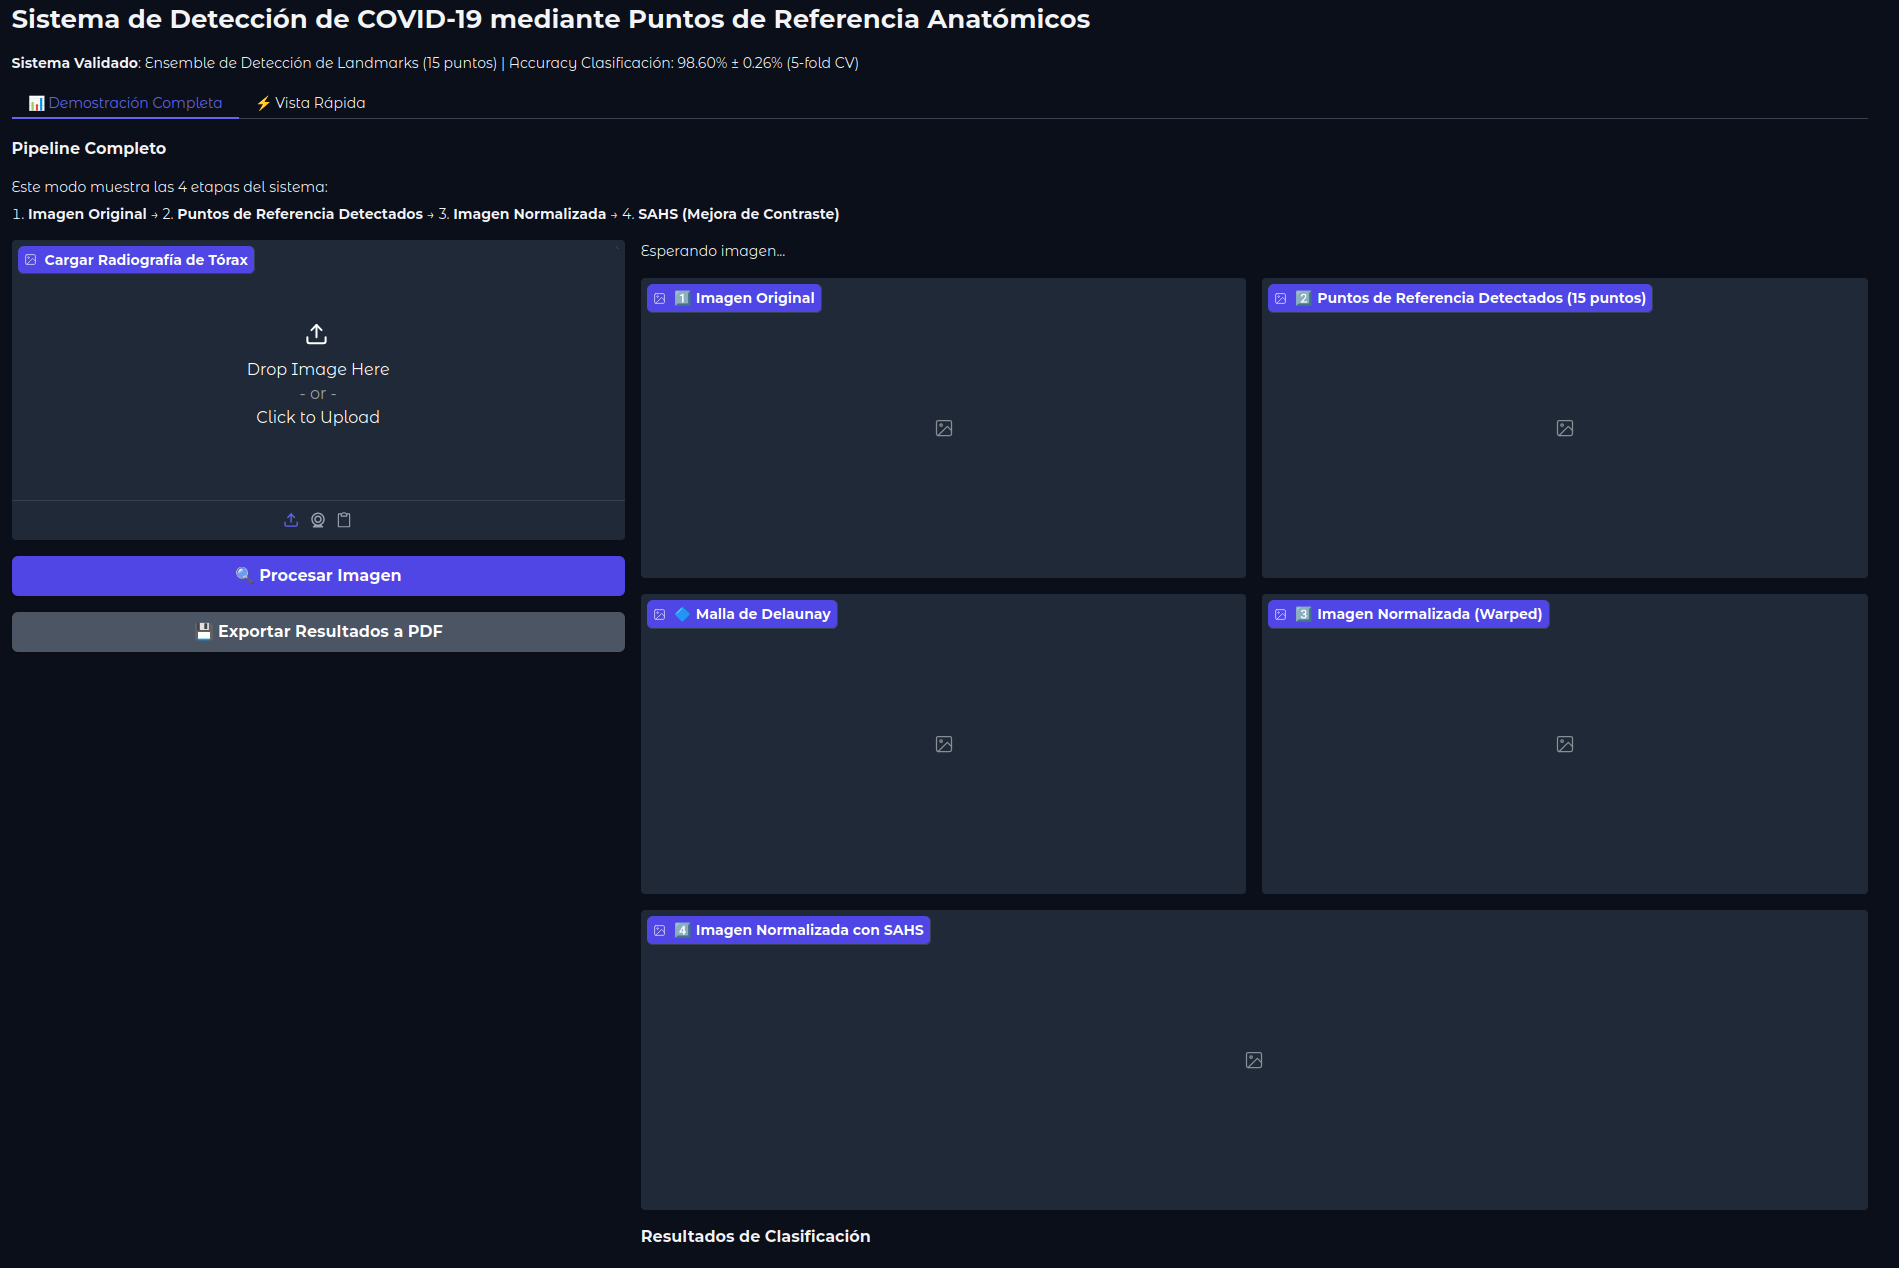
\includegraphics[width=0.9\textwidth]{imagenes/interfaz_principal.png}
\caption{Interfaz principal del sistema}
\label{fig:interfaz_principal}
\end{figure}

\newpage

% ============================================================================
% CAPÍTULO 2: INSTALACIÓN Y CONFIGURACIÓN
% ============================================================================
\section{Instalación y Configuración}

\subsection{Descarga del Sistema}

\paso{Paso 1:} Descargue el archivo del sistema desde el enlace proporcionado por su institución o investigador principal.

\paso{Paso 2:} El archivo se llama \texttt{covid19-demo-v15-portable-windows.zip} y tiene un tamaño aproximado de 600 MB.

\paso{Paso 3:} Guarde el archivo en una ubicación fácil de recordar, por ejemplo, en su escritorio o en la carpeta \texttt{Documentos}.

\subsection{Instalación}

\paso{Paso 1:} Haga clic derecho sobre el archivo ZIP descargado y seleccione \textbf{``Extraer todo...''} o \textbf{``Extract all...''}.

\begin{figure}[H]
\centering
\includegraphics[width=0.7\textwidth]{imagenes/extraer_zip.png}
\caption{Menú para extraer archivos en Windows}
\label{fig:extraer_zip}
\end{figure}

\paso{Paso 2:} Elija una carpeta de destino y haga clic en \textbf{``Extraer''}.

\paso{Paso 3:} Abra la carpeta extraída. Verá varios archivos y carpetas:

\begin{itemize}[leftmargin=*]
    \item \texttt{INSTALL.bat} -- Archivo de instalación
    \item \texttt{RUN\_DEMO.bat} -- Archivo para iniciar el sistema
    \item \texttt{README.txt} -- Información adicional
    \item Carpetas: \texttt{python}, \texttt{models}, \texttt{examples}, etc.
\end{itemize}

\paso{Paso 4:} Haga doble clic en el archivo \texttt{INSTALL.bat} para instalar las dependencias necesarias.

\nota{
La instalación puede tardar entre 5 y 10 minutos. Verá una ventana negra con texto desplazándose. No la cierre hasta que aparezca el mensaje ``Instalación completada'' o ``Installation completed''.
}

\begin{figure}[H]
\centering
\includegraphics[width=0.8\textwidth]{imagenes/instalacion.png}
\caption{Proceso de instalación en curso}
\label{fig:instalacion}
\end{figure}

\subsection{Inicio del Sistema}

\paso{Paso 1:} Una vez completada la instalación, haga doble clic en el archivo \texttt{RUN\_DEMO.bat}.

\paso{Paso 2:} Aparecerá una ventana negra con información sobre la carga del sistema. Espere de 10 a 15 segundos.

\paso{Paso 3:} Su navegador web predeterminado se abrirá automáticamente mostrando la interfaz del sistema en la dirección \texttt{http://localhost:7860}.

\consejo{
Si el navegador no se abre automáticamente, puede abrirlo manualmente y escribir \texttt{http://localhost:7860} en la barra de direcciones.
}

\begin{figure}[H]
\centering
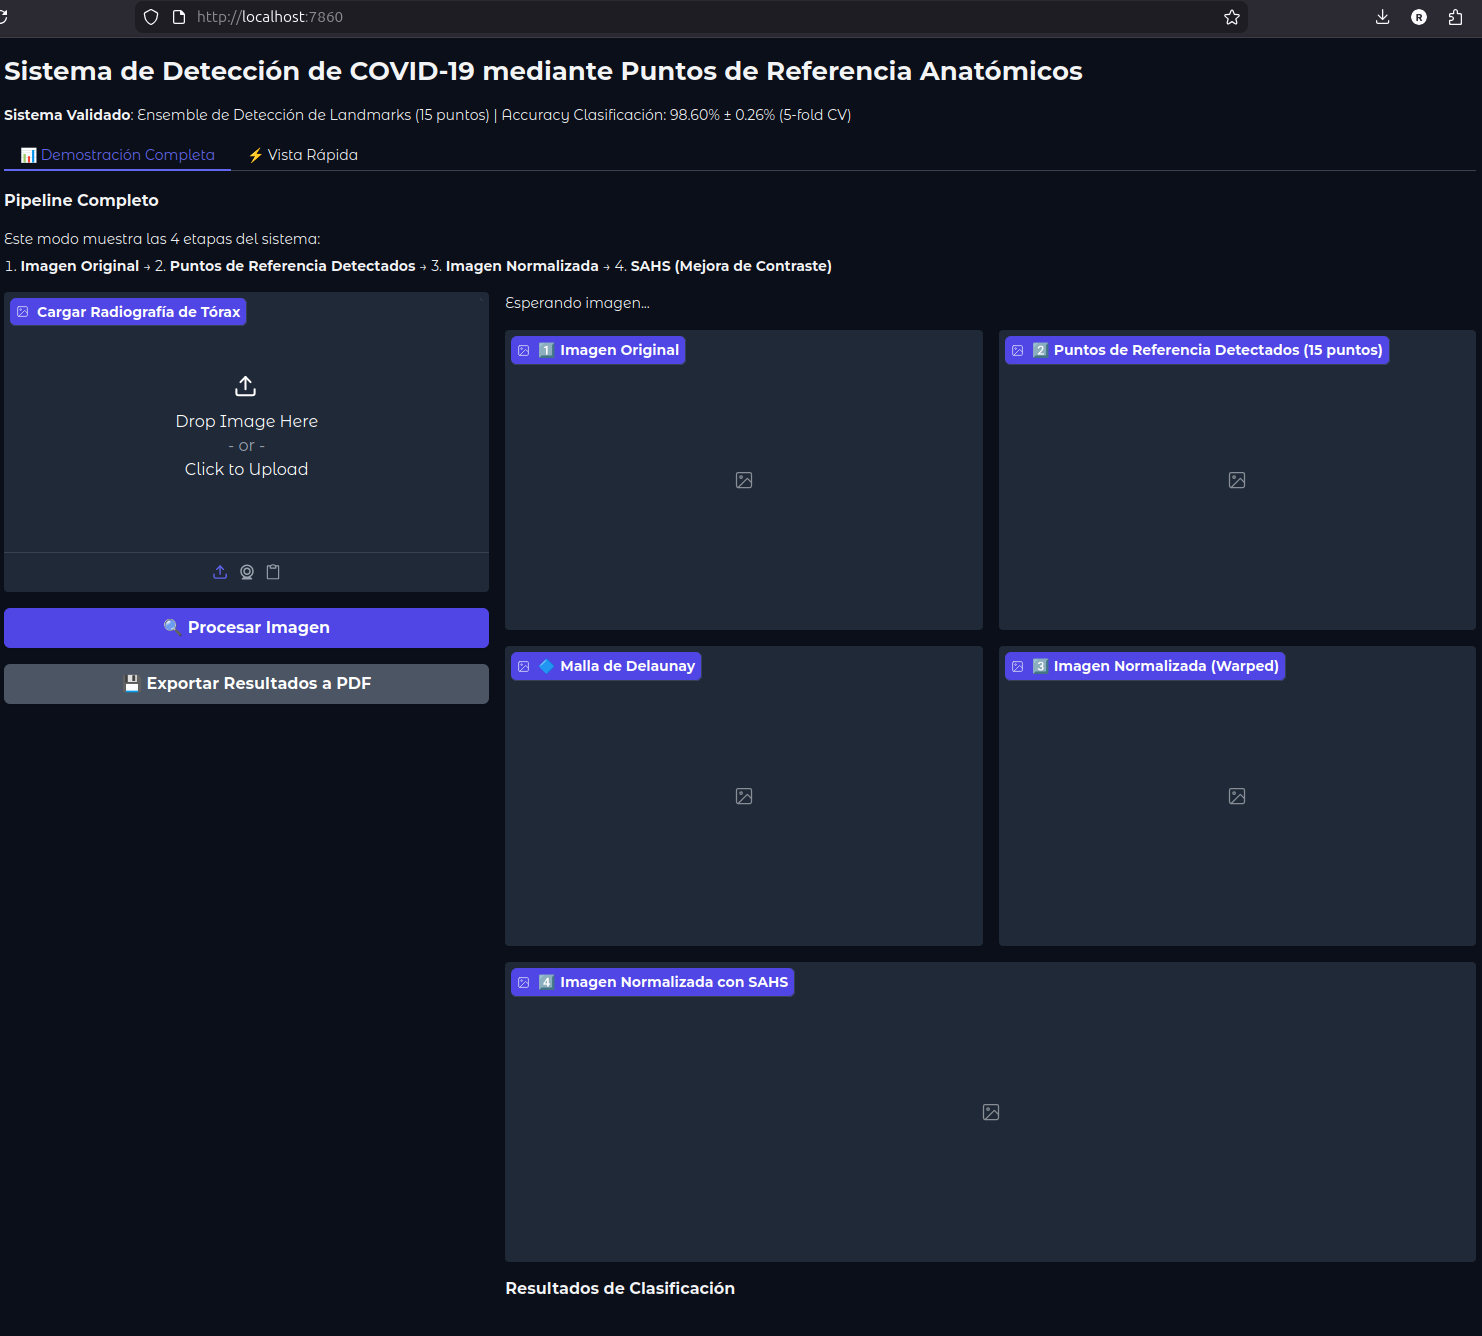
\includegraphics[width=0.9\textwidth]{imagenes/sistema_cargado.png}
\caption{Sistema cargado correctamente en el navegador}
\label{fig:sistema_cargado}
\end{figure}

\newpage

% ============================================================================
% CAPÍTULO 3: USO DEL SISTEMA - DEMOSTRACIÓN COMPLETA
% ============================================================================
\section{Uso del Sistema: Demostración Completa}

\subsection{Descripción de la Interfaz}

La interfaz del sistema tiene \textbf{dos pestañas principales}:

\begin{enumerate}[leftmargin=*]
    \item \textbf{Demostración Completa} -- Muestra todo el proceso paso a paso
    \item \textbf{Vista Rápida} -- Solo muestra el resultado final
\end{enumerate}

Comenzaremos con la \textbf{Demostración Completa}, que es la más educativa.

\subsection{Cargar una Radiografía}

\paso{Paso 1:} En la pestaña \textbf{``Demostración Completa''}, verá un área marcada como \textbf{``Cargar Radiografía de Tórax''} en el lado izquierdo.

\begin{figure}[H]
\centering
\includegraphics[width=0.8\textwidth]{imagenes/area_carga.png}
\caption{Área para cargar radiografías}
\label{fig:area_carga}
\end{figure}

\paso{Paso 2:} Haga clic en el área de carga o arrastre su imagen directamente.

\paso{Paso 3:} Seleccione una radiografía de tórax en formato PNG o JPG desde su computadora.

\consejo{
Si no tiene una radiografía disponible, el sistema incluye \textbf{ejemplos precargados} debajo del área de carga. Haga clic en cualquiera de ellos para probar el sistema.
}

\begin{figure}[H]
\centering
\includegraphics[width=0.9\textwidth]{imagenes/ejemplos.png}
\caption{Ejemplos precargados para prueba rápida}
\label{fig:ejemplos}
\end{figure}

\subsection{Procesar la Imagen}

\paso{Paso 1:} Una vez cargada la imagen, haga clic en el botón \boton{Procesar Imagen}.

\paso{Paso 2:} El sistema comenzará a analizar la radiografía. Verá un mensaje indicando que el procesamiento está en curso.

\paso{Paso 3:} El análisis completo toma aproximadamente \textbf{1 segundo}. Espere a que aparezcan los resultados.

\nota{
Durante el procesamiento, el sistema realiza varios pasos automáticos:
\begin{itemize}
    \item Detecta 15 puntos de referencia en los pulmones
    \item Normaliza la geometría de la imagen
    \item Analiza la radiografía normalizada
    \item Genera las visualizaciones
\end{itemize}
}

\subsection{Interpretación de Resultados}

Una vez completado el análisis, verá \textbf{cuatro imágenes principales}:

\subsubsection{1. Imagen Original}

Esta es la radiografía que usted cargó, tal como se ve originalmente.

\begin{figure}[H]
\centering
\includegraphics[width=0.7\textwidth]{imagenes/original.png}
\caption{Ejemplo de imagen original}
\label{fig:original}
\end{figure}

\subsubsection{2. Puntos de Referencia Detectados}

Muestra 15 puntos de colores sobre los pulmones. Estos puntos ayudan al sistema a identificar la estructura pulmonar:

\begin{itemize}[leftmargin=*]
    \item \textcolor{green}{\textbf{Puntos verdes}}: Parte superior e inferior del eje central
    \item \textcolor{cyan}{\textbf{Puntos celestes}}: Región central del pecho
    \item \textcolor{yellow}{\textbf{Puntos amarillos}}: Bordes laterales de los pulmones
    \item \textcolor{magenta}{\textbf{Puntos magentas}}: Parte superior de los pulmones
    \item \textcolor{red}{\textbf{Puntos rojos}}: Parte inferior de los pulmones
\end{itemize}

\begin{figure}[H]
\centering
\includegraphics[width=0.9\textwidth]{imagenes/landmarks.png}
\caption{Puntos de referencia detectados automáticamente}
\label{fig:landmarks}
\end{figure}

\consejo{
Los puntos del mismo color pertenecen a la misma región anatómica. Las líneas que los conectan muestran la simetría entre los pulmones izquierdo y derecho.
}

\subsubsection{Malla de Delaunay}

Muestra cómo el sistema divide la imagen en pequeños triángulos para normalizar la geometría. Esta es una visualización técnica que muestra el proceso interno.

\begin{figure}[H]
\centering
\includegraphics[width=0.8\textwidth]{imagenes/delaunay.png}
\caption{Malla de triangulación para normalización}
\label{fig:delaunay}
\end{figure}

\subsubsection{3. Imagen Normalizada}

Esta es la radiografía después de ajustar su geometría. Todas las radiografías se normalizan a la misma forma estándar, lo que permite una comparación más precisa.

\nota{
Notará que hay áreas negras alrededor de los pulmones. Esto es normal y es resultado del proceso de normalización geométrica.
}

\begin{figure}[H]
\centering
\includegraphics[width=0.7\textwidth]{imagenes/warped.png}
\caption{Imagen normalizada geométricamente}
\label{fig:warped}
\end{figure}

\subsubsection{4. Imagen con Mejora de Contraste}

Esta imagen tiene el contraste mejorado para resaltar mejor las estructuras pulmonares. El sistema utiliza una técnica llamada SAHS que mejora la visibilidad de detalles importantes.

\begin{figure}[H]
\centering
\includegraphics[width=0.7\textwidth]{imagenes/sahs.png}
\caption{Imagen con mejora de contraste SAHS}
\label{fig:sahs}
\end{figure}

\subsection{Resultado de la Clasificación}

Debajo de las cuatro imágenes, verá el \textbf{resultado principal}: la clasificación de la radiografía.

\subsubsection{Predicción Principal}

En un recuadro destacado con fondo oscuro, verá:
\begin{itemize}[leftmargin=*]
    \item Una estrella junto al diagnóstico predicho
    \item El nombre de la condición detectada en color:
    \begin{itemize}
        \item \textcolor{covidred}{\textbf{COVID-19}} (en rojo)
        \item \textcolor{normalgreen}{\textbf{Normal}} (en verde)
        \item \textcolor{virusyellow}{\textbf{Neumonía Viral}} (en amarillo)
    \end{itemize}
\end{itemize}

\begin{figure}[H]
\centering
\includegraphics[width=0.6\textwidth]{imagenes/prediccion.png}
\caption{Predicción principal destacada}
\label{fig:prediccion}
\end{figure}

\subsubsection{Probabilidades por Clase}

Debajo de la predicción, verá tres barras de colores que indican la confianza del sistema en cada categoría:

\begin{itemize}[leftmargin=*]
    \item Cada barra muestra un porcentaje (0\% a 100\%)
    \item La clase con el porcentaje más alto es la predicción del sistema
    \item La suma de los tres porcentajes siempre es 100\%
\end{itemize}

\begin{figure}[H]
\centering
\includegraphics[width=0.8\textwidth]{imagenes/probabilidades.png}
\caption{Barras de probabilidad por clase}
\label{fig:probabilidades}
\end{figure}

\subsubsection{Interpretación de las Probabilidades}

\begin{itemize}[leftmargin=*]
    \item \textbf{90-100\%:} El sistema tiene muy alta confianza
    \item \textbf{70-90\%:} El sistema tiene alta confianza
    \item \textbf{50-70\%:} El sistema tiene confianza moderada
    \item \textbf{33-50\%:} El sistema tiene baja confianza
    \item \textbf{Menos de 33\%:} El sistema no detecta claramente esa condición
\end{itemize}

\advertencia{
Incluso con porcentajes altos, los resultados deben ser \textbf{siempre} verificados por un médico profesional. Este sistema es una herramienta de apoyo, no un sustituto del diagnóstico médico.
}

\subsection{Métricas Detalladas (Opcional)}

Si desea ver información técnica adicional:

\paso{Paso 1:} Haga clic en el acordeón \textbf{``Métricas Detalladas''}.

\paso{Paso 2:} Verá una tabla con las coordenadas exactas de los 15 puntos detectados.

\paso{Paso 3:} También verá el tiempo que tardó el análisis (generalmente alrededor de 1 segundo).

\begin{figure}[H]
\centering
\includegraphics[width=0.9\textwidth]{imagenes/metricas.png}
\caption{Métricas detalladas expandidas}
\label{fig:metricas}
\end{figure}

\subsection{Exportar Resultados a PDF}

Si desea guardar los resultados para compartirlos o archivarlos:

\paso{Paso 1:} Haga clic en el botón \boton{Exportar Resultados a PDF}.

\paso{Paso 2:} El sistema generará un archivo PDF con todas las imágenes y resultados.

\paso{Paso 3:} El archivo se guardará en la carpeta del sistema con un nombre que incluye la fecha y hora (por ejemplo: \texttt{resultado\_20260127\_143025.pdf}).

\paso{Paso 4:} Verá un mensaje confirmando la exportación exitosa con la ruta del archivo.

\consejo{
El PDF generado incluye todas las visualizaciones y una tabla con las coordenadas de los puntos, ideal para documentación o presentaciones.
}

\newpage

% ============================================================================
% CAPÍTULO 4: USO DEL SISTEMA - VISTA RÁPIDA
% ============================================================================
\section{Uso del Sistema: Vista Rápida}

\subsection{¿Cuándo Usar la Vista Rápida?}

Use la pestaña \textbf{``Vista Rápida''} cuando:
\begin{itemize}[leftmargin=*]
    \item Solo necesita conocer el diagnóstico sin ver el proceso
    \item Desea analizar varias radiografías rápidamente
    \item Ya está familiarizado con el sistema
\end{itemize}

\subsection{Proceso Simplificado}

\paso{Paso 1:} Cambie a la pestaña \textbf{``Vista Rápida''}.

\begin{figure}[H]
\centering
\includegraphics[width=0.9\textwidth]{imagenes/vista_rapida.png}
\caption{Interfaz de Vista Rápida}
\label{fig:vista_rapida}
\end{figure}

\paso{Paso 2:} Cargue su radiografía (igual que en la Demostración Completa).

\paso{Paso 3:} Haga clic en el botón \boton{Clasificar}.

\paso{Paso 4:} Verá directamente:
\begin{itemize}
    \item La predicción destacada con la estrella
    \item Las barras de probabilidad
    \item El tiempo de análisis
\end{itemize}

\nota{
La Vista Rápida es aproximadamente \textbf{2 veces más rápida} que la Demostración Completa porque no genera las visualizaciones intermedias.
}

\newpage

% ============================================================================
% CAPÍTULO 5: SOLUCIÓN DE PROBLEMAS
% ============================================================================
\section{Solución de Problemas Comunes}

\subsection{El sistema no inicia}

\textbf{Problema:} Al hacer doble clic en \texttt{RUN\_DEMO.bat}, nada sucede.

\textbf{Soluciones:}
\begin{enumerate}[leftmargin=*]
    \item Verifique que completó la instalación con \texttt{INSTALL.bat}
    \item Cierre todas las ventanas y vuelva a intentar
    \item Reinicie su computadora e intente nuevamente
    \item Asegúrese de que no hay otro programa usando el puerto 7860
\end{enumerate}

\subsection{La página no carga en el navegador}

\textbf{Problema:} El navegador muestra un error ``No se puede acceder al sitio''.

\textbf{Soluciones:}
\begin{enumerate}[leftmargin=*]
    \item Espere 15-20 segundos adicionales (la carga inicial puede tardar)
    \item Verifique que la ventana negra (terminal) sigue abierta
    \item Intente cerrar el navegador y volver a abrirlo manualmente escribiendo \texttt{http://localhost:7860}
    \item Verifique su firewall o antivirus, podría estar bloqueando la conexión
\end{enumerate}

\subsection{El procesamiento es muy lento}

\textbf{Problema:} El análisis tarda más de 5 segundos.

\textbf{Explicación:} El sistema funciona más rápido con una tarjeta gráfica (GPU), pero también puede funcionar solo con el procesador (CPU), aunque será más lento.

\textbf{Soluciones:}
\begin{enumerate}[leftmargin=*]
    \item Use la Vista Rápida en lugar de la Demostración Completa
    \item Cierre otros programas que consuman recursos
    \item Sea paciente: 3-5 segundos es normal en computadoras sin GPU dedicada
\end{enumerate}

\subsection{Error al cargar la imagen}

\textbf{Problema:} Aparece un mensaje de error al intentar cargar una imagen.

\textbf{Soluciones:}
\begin{enumerate}[leftmargin=*]
    \item Verifique que la imagen está en formato PNG o JPG
    \item Asegúrese de que la imagen no esté corrupta (intente abrirla con otro programa primero)
    \item Si la imagen es muy grande (más de 5 MB), intente reducir su tamaño
    \item Verifique que la imagen sea realmente una radiografía de tórax
\end{enumerate}

\subsection{Resultados inesperados}

\textbf{Problema:} El sistema da un resultado que parece incorrecto.

\textbf{Consideraciones:}
\begin{enumerate}[leftmargin=*]
    \item El sistema es una herramienta de apoyo, no un diagnóstico definitivo
    \item La calidad de la radiografía afecta los resultados
    \item Radiografías con ángulos inusuales pueden dar resultados menos precisos
    \item Si la confianza es baja (menos del 70\%), el sistema mismo indica incertidumbre
    \item Consulte siempre con un profesional médico
\end{enumerate}

\subsection{Mensajes de advertencia}

Si ve alguno de estos mensajes:

\begin{itemize}[leftmargin=*]
    \item \textbf{``Warping falló, mostrando imagen original'':} El sistema no pudo normalizar la geometría, pero el análisis continuó con la imagen original. Los resultados pueden ser menos precisos.

    \item \textbf{``GPU sin memoria suficiente'':} El sistema cambió automáticamente a usar el procesador (CPU). El análisis será un poco más lento pero funcionará correctamente.

    \item \textbf{``Formato no soportado'':} La imagen debe estar en formato PNG o JPG. Convierta su imagen y vuelva a intentar.
\end{itemize}

\newpage

% ============================================================================
% CAPÍTULO 6: PREGUNTAS FRECUENTES
% ============================================================================
\section{Preguntas Frecuentes}

\subsection{¿Puedo usar este sistema para diagnosticar pacientes?}

\textbf{No.} Este sistema es una herramienta de investigación y apoyo académico. \textbf{No está diseñado ni aprobado} para uso clínico directo. Todos los resultados deben ser interpretados y validados por profesionales médicos certificados.

\subsection{¿Qué tan preciso es el sistema?}

El sistema tiene una precisión del 98.60\% en pruebas con imágenes del conjunto de datos de entrenamiento. Sin embargo, la precisión puede variar con:
\begin{itemize}[leftmargin=*]
    \item Calidad de la radiografía
    \item Equipo usado para tomar la radiografía
    \item Posición del paciente
    \item Condiciones que no fueron parte del entrenamiento
\end{itemize}

\subsection{¿Puedo procesar múltiples imágenes a la vez?}

Actualmente, el sistema procesa una imagen a la vez. Para analizar múltiples imágenes:
\begin{enumerate}[leftmargin=*]
    \item Procese la primera imagen
    \item Si desea guardar los resultados, use ``Exportar a PDF''
    \item Cargue la siguiente imagen
    \item Repita el proceso
\end{enumerate}

\subsection{¿Puedo usar radiografías de otras partes del cuerpo?}

\textbf{No.} El sistema está específicamente entrenado para radiografías de tórax. Si carga otro tipo de imagen médica (abdomen, extremidades, etc.), los resultados no serán válidos.

\subsection{¿Funciona con radiografías de niños?}

El sistema fue entrenado principalmente con radiografías de adultos. Los resultados con radiografías pediátricas pueden ser menos precisos debido a las diferencias anatómicas.

\subsection{¿Necesito estar conectado a internet para usar el sistema?}

\textbf{No.} Una vez instalado, el sistema funciona completamente \textbf{sin conexión a internet}. Todos los modelos y componentes están incluidos en el paquete descargado.

\subsection{¿Los datos de las radiografías se envían a algún servidor?}

\textbf{No.} Todo el procesamiento se realiza \textbf{localmente en su computadora}. Las imágenes nunca se envían a internet ni se almacenan en servidores externos.

\subsection{¿Puedo cerrar el navegador sin detener el sistema?}

Sí. Si cierra el navegador, el sistema sigue ejecutándose. Para volver a acceder, simplemente:
\begin{enumerate}[leftmargin=*]
    \item Abra su navegador
    \item Escriba \texttt{http://localhost:7860}
    \item Presione Enter
\end{enumerate}

Para detener completamente el sistema, cierre la ventana negra (terminal).

\subsection{¿Cuánto espacio ocupa el sistema en mi disco?}

Aproximadamente 1.5 GB:
\begin{itemize}[leftmargin=*]
    \item Archivo descargado (ZIP): 600 MB
    \item Archivos extraídos: 900 MB adicionales
\end{itemize}

\newpage

% ============================================================================
% CAPÍTULO 7: GLOSARIO DE TÉRMINOS
% ============================================================================
\section{Glosario de Términos}

\begin{description}[leftmargin=2cm,style=nextline]

\item[Radiografía de tórax] Imagen médica que muestra los pulmones, corazón y estructuras del pecho, tomada con rayos X.

\item[COVID-19] Enfermedad respiratoria causada por el coronavirus SARS-CoV-2. Puede causar neumonía y otros síntomas respiratorios graves.

\item[Neumonía Viral] Infección de los pulmones causada por un virus (no necesariamente COVID-19). Puede ser causada por influenza, adenovirus u otros virus.

\item[Puntos de referencia (Landmarks)] Puntos específicos detectados automáticamente por el sistema que marcan ubicaciones importantes en los pulmones.

\item[Normalización geométrica] Proceso de ajustar todas las radiografías a una forma estándar para permitir comparaciones más precisas.

\item[Confianza] Porcentaje que indica qué tan seguro está el sistema de su predicción. Mayor porcentaje = mayor confianza.

\item[Inteligencia Artificial (IA)] Tecnología que permite a las computadoras aprender a realizar tareas complejas analizando ejemplos.

\item[GPU (Tarjeta Gráfica)] Componente de hardware que acelera el procesamiento de imágenes. El sistema funciona más rápido si su computadora tiene una GPU dedicada.

\item[CPU (Procesador)] El cerebro de la computadora. El sistema puede funcionar solo con CPU, pero será más lento que con GPU.

\item[Localhost] Dirección especial (\texttt{http://localhost:7860}) que se refiere a su propia computadora. Cuando accede a esta dirección, está accediendo a un programa que corre localmente.

\item[PDF] Formato de documento portable que preserva el formato de las imágenes y texto. Los resultados exportados se guardan en este formato.

\item[PNG/JPG] Formatos de imagen digital. PNG es sin pérdida de calidad, JPG usa compresión. Ambos son aceptados por el sistema.

\end{description}

\newpage

% ============================================================================
% CAPÍTULO 8: INFORMACIÓN DE CONTACTO Y SOPORTE
% ============================================================================
\section{Información de Contacto}

\subsection{Soporte Técnico}

Si encuentra problemas técnicos que no se resuelven con este manual:

\begin{enumerate}[leftmargin=*]
    \item Revise el archivo \texttt{README.txt} incluido en la carpeta del sistema
    \item Contacte al investigador principal o supervisor de su institución
    \item Proporcione la siguiente información al reportar problemas:
    \begin{itemize}
        \item Versión del sistema (Versión 15)
        \item Sistema operativo (Windows 10, Windows 11, etc.)
        \item Descripción detallada del problema
        \item Mensaje de error exacto (si aparece alguno)
        \item Captura de pantalla del problema
    \end{itemize}
\end{enumerate}

\subsection{Uso Académico}

Este sistema fue desarrollado como parte de una investigación académica. Si desea:
\begin{itemize}[leftmargin=*]
    \item Citar este sistema en publicaciones
    \item Obtener más información sobre la metodología
    \item Solicitar acceso a los datos de entrenamiento
    \item Colaborar en investigación relacionada
\end{itemize}

Por favor contacte al investigador principal a través de su institución académica.

\subsection{Reporte de Errores}

Si identifica un comportamiento incorrecto del sistema:
\begin{enumerate}[leftmargin=*]
    \item Documente el problema con capturas de pantalla
    \item Guarde la radiografía que causó el problema (si es posible)
    \item Anote los pasos exactos que siguió
    \item Reporte al supervisor o investigador principal
\end{enumerate}

\nota{
Su retroalimentación es valiosa para mejorar el sistema. No dude en reportar cualquier comportamiento inesperado.
}

\newpage

% ============================================================================
% CAPÍTULO 9: ANEXOS
% ============================================================================
\section{Anexos}

\subsection{Anexo A: Lista de Verificación Pre-Análisis}

Antes de analizar una radiografía, verifique:

\begin{itemize}[itemsep=3pt]
    \item[$\square$] La imagen es una radiografía de tórax (no otra parte del cuerpo)
    \item[$\square$] La imagen está en formato PNG o JPG
    \item[$\square$] La radiografía fue tomada de frente (vista posteroanterior o anteroposterior)
    \item[$\square$] La imagen no está rotada ni invertida
    \item[$\square$] La calidad de la imagen es suficiente (no muy borrosa ni pixelada)
    \item[$\square$] El sistema está correctamente iniciado (navegador abierto en localhost:7860)
\end{itemize}

\subsection{Anexo B: Interpretación de Colores}

Tabla de referencia rápida para los colores del sistema:

\begin{table}[H]
\centering
\begin{tabular}{|l|l|p{6cm}|}
\hline
\textbf{Color} & \textbf{Significado} & \textbf{Contexto} \\
\hline
\textcolor{covidred}{\textbf{Rojo}} & COVID-19 & Clasificación predicha o barra de probabilidad \\
\hline
\textcolor{normalgreen}{\textbf{Verde}} & Normal & Clasificación predicha o barra de probabilidad \\
\hline
\textcolor{virusyellow}{\textbf{Amarillo}} & Neumonía Viral & Clasificación predicha o barra de probabilidad \\
\hline
\textcolor{green}{\textbf{Verde brillante}} & Eje vertical & Puntos de referencia (L1, L2) \\
\hline
\textcolor{cyan}{\textbf{Celeste}} & Región central & Puntos de referencia (L9, L10, L11) \\
\hline
\textcolor{yellow}{\textbf{Amarillo}} & Bordes laterales & Puntos de referencia (L3-L8) \\
\hline
\textcolor{magenta}{\textbf{Magenta}} & Ápices superiores & Puntos de referencia (L12, L13) \\
\hline
\textcolor{red}{\textbf{Rojo}} & Ángulos inferiores & Puntos de referencia (L14, L15) \\
\hline
\end{tabular}
\caption{Referencia de colores del sistema}
\end{table}

\subsection{Anexo C: Especificaciones Técnicas del Sistema}

Para usuarios con conocimientos técnicos:

\begin{itemize}[leftmargin=*]
    \item \textbf{Versión del sistema:} 15 (v1.0.10)
    \item \textbf{Fecha de construcción:} 21 de enero de 2026
    \item \textbf{Framework:} Gradio 6.3.0
    \item \textbf{Python:} 3.12.8
    \item \textbf{Modelos:}
    \begin{itemize}
        \item Ensemble de landmarks: 4 modelos ResNet-18
        \item Clasificador: ResNet-18 finetuned
    \end{itemize}
    \item \textbf{Precisión validada:}
    \begin{itemize}
        \item Error de landmarks: 3.61 ± 2.48 píxeles
        \item Accuracy clasificación: 98.60\% ± 0.26\%
        \item F1-Score macro: 98.00\% ± 0.36\%
    \end{itemize}
    \item \textbf{Tiempo de inferencia:} ~1 segundo (con GPU)
    \item \textbf{Tamaño de entrada:} 224×224 píxeles
\end{itemize}

\newpage

\subsection{Anexo D: Captura de Pantalla Completa Anotada}

\begin{figure}[H]
\centering
\includegraphics[width=0.95\textwidth]{imagenes/interfaz_anotada.png}
\caption{Vista completa de la interfaz con elementos principales identificados}
\label{fig:interfaz_anotada}
\end{figure}

\newpage

% ============================================================================
% PÁGINA FINAL
% ============================================================================

\section*{Acerca de Este Manual}

\subsection*{Versión del Manual}
Este es el Manual de Usuario versión 1.0, correspondiente al Sistema de Detección de COVID-19 versión 15, publicado en enero de 2026.

\subsection*{Propósito}
Este manual fue diseñado específicamente para usuarios sin conocimientos técnicos, con el objetivo de hacer el sistema accesible para:
\begin{itemize}[leftmargin=*]
    \item Personal médico sin experiencia en informática
    \item Estudiantes de ciencias de la salud
    \item Investigadores de áreas no técnicas
    \item Cualquier persona interesada en utilizar el sistema
\end{itemize}

\subsection*{Agradecimientos}
Este sistema es el resultado de una investigación académica en el campo de la inteligencia artificial aplicada a imágenes médicas. Agradecemos a todos los que contribuyeron al desarrollo y validación del sistema.

\vspace{1cm}

\begin{center}
\rule{0.5\textwidth}{0.5pt}
\end{center}

\vspace{0.5cm}

\begin{center}
\textbf{Sistema de Detección de COVID-19}\\
Versión 15 -- Enero 2026\\[0.3cm]
\textit{Herramienta de Apoyo para Investigación Académica}\\[0.3cm]
\textbf{NO es un dispositivo médico aprobado para diagnóstico clínico}
\end{center}

\vspace{1cm}

\begin{center}
\rule{0.5\textwidth}{0.5pt}
\end{center}

\end{document}
